% !TEX encoding = UTF-8 Unicode
% !TEX program = pdflatex
% !TEX spellcheck = en_US


% In order to correctly compile this document,
% execute the following commands:
% 1. pdflatex
% 2. pdflatex
% 3. pdflatex



\documentclass[amsthm,ebook]{saparticle}

% IF YOU USE PDFLATEX
\usepackage[utf8x]{inputenc}
% if you write in english and in greek
\usepackage{ucs}
\usepackage[greek,english]{babel}
\languageattribute{greek}{polutoniko}

% IF YOU USE XELATEX
%\usepackage{polyglossia}
% if you write in italian
%\setmainlanguage{italian}
% If you want put some ancient greek:
%\setotherlanguage[variant=polytonic]{greek}
%\newfontfamily{\greekfont}[Ligatures=TeX]{Palatino Linotype}

% dummy text (remove in a normal thesis)
% remove if not necessary
\usepackage{siunitx}
%Natbib for bibliography management
\usepackage[authoryear]{natbib}
% custom commands
\newcommand{\bs}{\textbackslash}

%%%%%%%%
%TITLE:%
%%%%%%%%
\title{AXON. A Selection of Greek Historical Inscriptions. A Database for Research and Teaching}
 \author[cafo]{Ivan Matijašić\corref{first}}
\author[cafo]{Stefania De Vido}
\author[cafo]{Silvia Palazzo}
\address[cafo]{Dipartimento di Studi Umanistici, Università Ca' Foscari Venezia}
\cortext[first]{Corresponding author. Email: ivan.matijasic@unive.it}
\begin{document}

\maketitle
\begin{abstract}
The AXON Project has developed a database of Greek historical inscriptions, from the birth of the~polis~in the Archaic
Age to 31 BC. Each entry is provided with the object’s description, a complete lemma, Greek text with critical
apparatus, Italian translation and commentary with keywords and indexes, and updated bibliography. New insights for
data-inclusion have been developed. The database supports enlargement and offers a high degree of searchability. Our
aim is to illustrate the structure, the contents and the solutions we have come up with in the development of the AXON
Project. We will also offer some suggestions for teaching and academic research purposes.


\end{abstract}
\keywords{Online epigraphic editions; interoperability of digital editions of Greek historical inscriptions; images of Greek
historical inscriptions; digital epigraphy in teaching and research}




\section{The AXON Project }


AXON. A Selection of Greek Historical Inscriptions is a project conceived within the Greek Epigraphy Laboratory
(Director, Prof. Claudia Antonetti), and has been brought into existence with the financial support of the University
Ca’ Foscari of Venice (University Project 2013, Project Coordinator, Prof. Stefania De Vido).

Since October 2014 the members of the AXON Project have been developing a database which includes a great variety of
Greek inscriptions of different chronology, typology, and territory of origin. The most recent advances of traditional
epigraphy as well as the scientific acquisitions in the Digital Humanities have been taken into account. The selection
of texts has been made according to a broader notion of ‘historical’ inscription, including not only significant
military, political, and institutional texts, but also those inscriptions which are essential for the social and
cultural understanding of the Greek world. 

AXON includes texts from the birth of the Greek polis in the Archaic Age\footnote{ See the Introduction in \citet{nielsen_inventory_2004}; \citet{hansen_polis:_2006}. } to 31 BC, a chronological frame traditionally related to Greek History (though a future
extension of this chronological limit is not excluded). The epigraphic entries have been prearranged in order to allow
a wide and well-structured description of each document. At the same time, a common and coherent lexicon has been
produced, which will permit an easier indexing of significant words and will make future searches much quicker. 




\section{A unique model-entry for a great diversity of inscriptions: taxonomy and categorisation}





\subsection{Entry description}

\subsubsection{Object’s description}


The model-entry has been created with an eye on the object’s thorough description. Here is the object’s categorisation:

\begin{enumerate}
\item Object type
\item Material
\item Object’s dimensions
\item State of preservation
\item Further descriptive elements
\item Date and context of finding
\item Finding site (modern nation, ancient region, ancient and modern name of the city, if known)
\item Actual location (modern nation, city, museum/archaelogical context, inventory number)
\end{enumerate}
The great majority of these categories can be selected from a given number of options from a pull-down menu. Some
categories – such as Object type, Material, or State of preservation – are directly linked with the corresponding
sections in the EAGLE Vocabularies (see \url{http://www.eagle-network.eu/resources/vocabularies/}). Furthermore, a hyperlink
has been created between the AXON-entries and Pleiades website (\url{http://pleiades.stoa.org}): where the finding site is
known, each entry offers the geographic coordinates and a Googlemaps visualisation. This gives the possibility of
rapidly gathering the information for any single ancient location and allows for searches directly from an interactive
map.




\subsubsection{Chronology}


The chronological delimitation of each text is supported by many options, as you can see in Fig.~\ref{fig:1}:

\begin{figure}[!bp]
\centering
 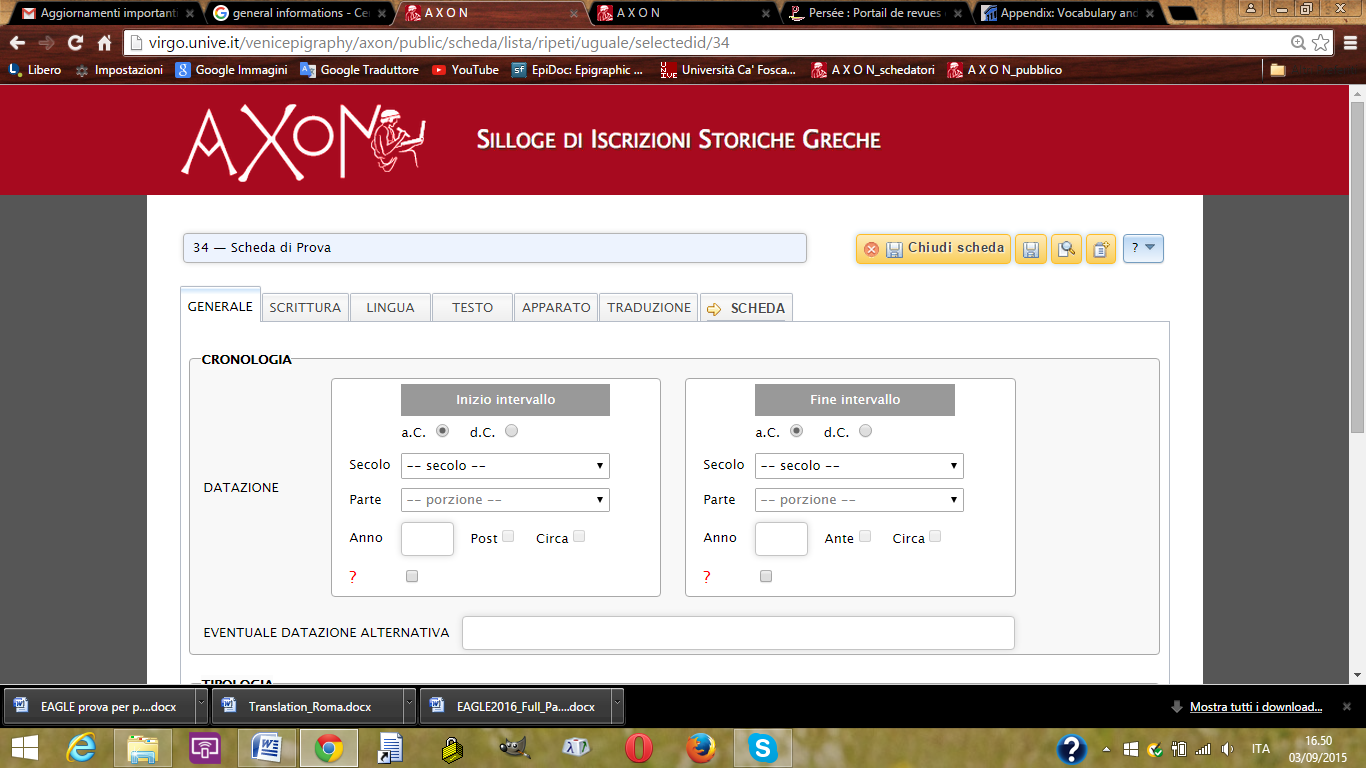
\includegraphics[width=\columnwidth]{EAGLE2016FullPaperrevised-img001.png}
\caption{Window for the input of data, section Text/Chronology}
\label{fig:1}
\end{figure}




\subsubsection{Alphabet \& language}





Each entry provides all the necessary information on the alphabet and language of each inscription:

\begin{enumerate}
\item Type of Inscription (with link to EAGLE’s Vocabularies:
\url{http://www.eagle-network.eu/resources/vocabularies/typeins/}. The categories are those used by \citet{guarducci_epigrafia_1987})
\item Text’s structure
\item Writing (Execution technique\footnote{ With link to \url{http://www.eagle-network.eu/resources/vocabularies/writing/}.};
different types of epichoric alphabets according to Kirchhoff’s colour-coded map; Local script\footnote{ Following the
categorisation in \citet{jeffery_local_1990}.}; Palaeographic features and letters’ form\footnote{ The letter-form and glyph-form are
based on the symbols of the font Cardo (\url{http://scholarsfonts.net/cardofnt.html}), but many have been developed by the
AXON Team on the examples of letter-form given in Jeffrey 1990 (see also
\url{http://poinikastas.csad.ox.ac.uk/browseGlyphs.shtml}).}; letters’ heights, description and layout of the text field;
Direction of Text)
\item Language (with an option for any dialect’s peculiarities)
\end{enumerate}






\subsubsection{Genetic lemma \& apparatus criticus}


The text of each inscription is preceded by a hierarchically arranged lemma (the so called genetic lemma, according to
Louis Robert’s definition\footnote{\citet{robert_carie:_1954}.}) and is followed by the apparatus criticus.




\subsubsection{Italian translation \& commentary}


Each entry corresponds to an Italian translation and commentary (in .pdf). 




\subsubsection{Abstract}


The Abstract – with a WYSIWYG interface – includes all the keywords for indexing and lemmatisation:

\begin{figure}[!bp]
\centering
 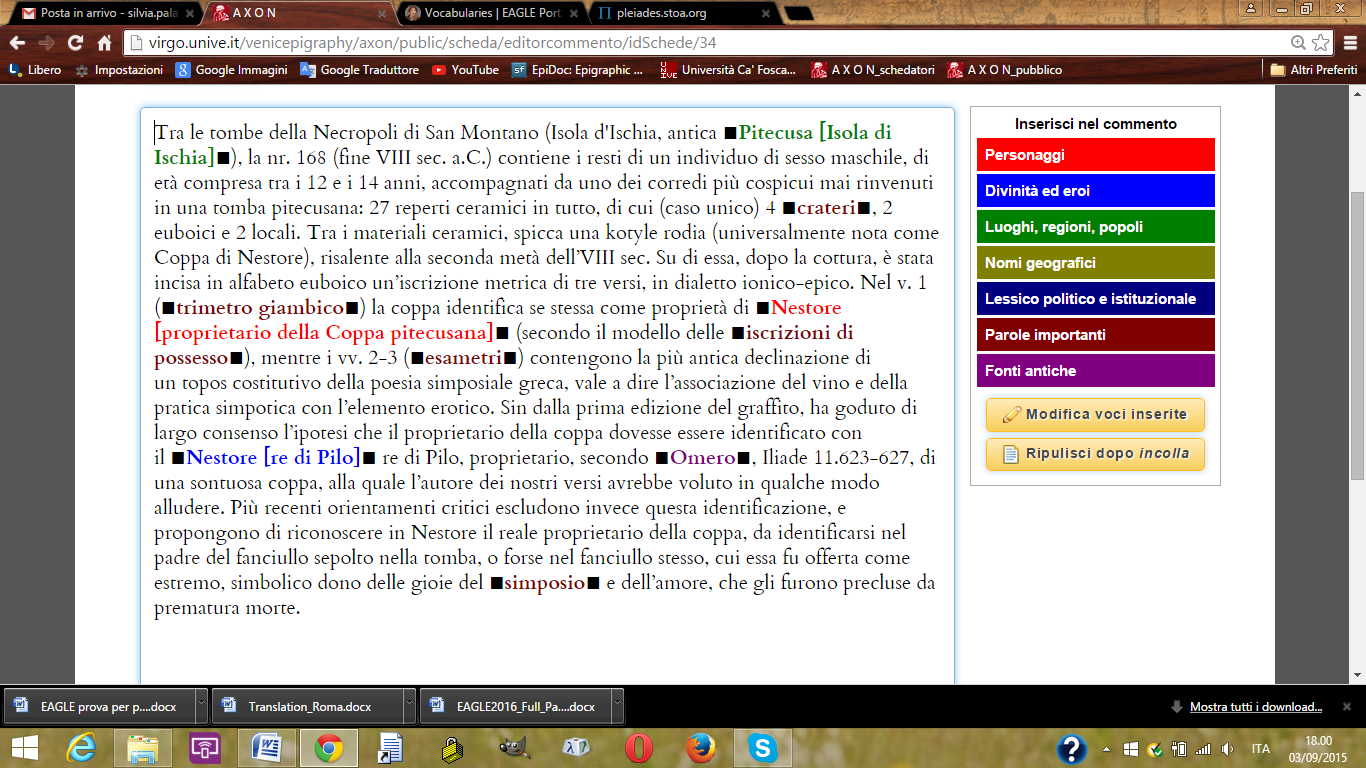
\includegraphics[width=\columnwidth]{EAGLE2016FullPaperrevised-img002.png}
\caption{Example of Abstract in AXON. The different colours allow a selection of words from a drop-down menu. }
\label{fig:2}
\end{figure}




The Keywords are divided into the following categories (these categories are based on EpiDoc Community Guidelines as
well as on the indexes of the Supplementum Epigraphicum Graecum, SEG):

\begin{enumerate}
\item Persons and names (mainly for ‘historical’ characters)
\item Gods and heroes
\item Place names
\item Geographical names
\item Significant words regarding the history of politics and institutions
\item Other relevant keywords
\item Ancient sources
\end{enumerate}



\subsubsection{Bibliography}


Finally, an updated bibliography highlights any previous edition for each entry, as well as all the appropriate
secondary sources. SEG abbreviations have been used for epigraphic corpora and other publications (the section
``materiali'' on the website gives access to a list of all abbreviations, useful for students, as well\footnote{
\url{http://virgo.unive.it/venicepigraphy/axon/public/axon/pagine/materiali} (still being processed).}).




\subsection{Internal \& external interoperability of the AXON database}





Each entry is related – whenever it seems appropriate – to other entries in the AXON database. A hyperlink connects the
entry with other digital editions of the same text (if available), or with other useful websites, possibly containing
images. Wherever possible, images and/or apographs and/or squeezes of inscriptions have been included. The creation of
a digital archive of images as part of the AXON website is also desirable.




\subsection{A simple website interface for the input of data}





Since the contributors to the project (i.e. the authors of the entries) are experts from different Italian and European
universities (and not all of them are familiar with the Digital Humanities), and given the great number of entries
planned in the near future, the necessity of a simple and easily understandable interface for the input of data was an
essential issue to the project from the very beginning. Guidelines to EpiDoc have been taken into account in order to
produce a clear structure for the input of data.

Our aim is to establish a growing community of experts, students, and enthusiasts to increase the number of contributors
through lists of inscriptions which have not yet been assigned. At the same time it will be the possible to suggest
other texts which are not included in the lists. To achieve these aims, the project follows an EpiDoc-friendly
structure and is compatible with Europeana EAGLE Project, especially in the use of a common terminology. 







\section{Searchability}





The website is designed to allow for many search options. Beyond the ``full text'' search and another based on the number,
title and author of the entry (see Fig.~\ref{fig:3}), three other search-possibilities will also be available:

\begin{figure}[!bp]
\centering
 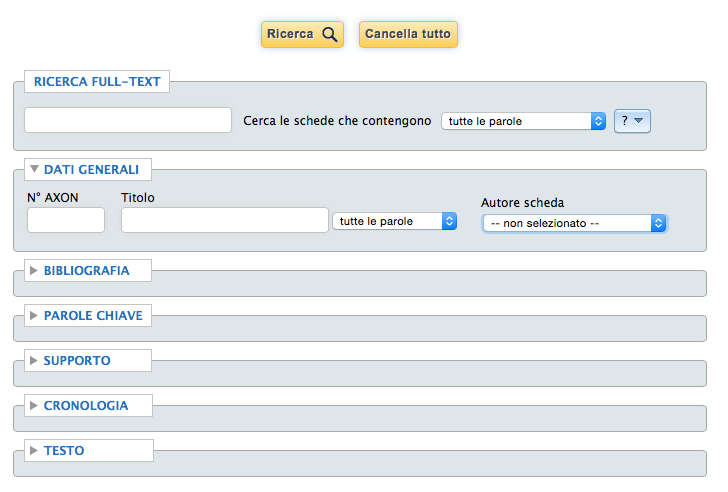
\includegraphics[width=\columnwidth]{EAGLE2016FullPaperrevised-img003.png}
\caption{Search based on ``Full text'', number, title, and author of the entry.}
\label{fig:3}
\end{figure}



\begin{enumerate}
\item browse all the entries according to the inscriptions’ a) typology, b) chronology, and c) area of origin;
\item access the entries through an interactive map;
\item perform an advanced search based on different categories: 
\begin{enumerate}
\item bibliography
\item keywords
\item object’s description and preservation (see Fig.~\ref{fig:4})
\item chronology
\item text (single words or phrases, typology, dialect, alphabet, letter-form, etc.) (see Fig.~\ref{fig:5}).
\end{enumerate}
\end{enumerate}







\begin{figure}[!bp]
\centering
 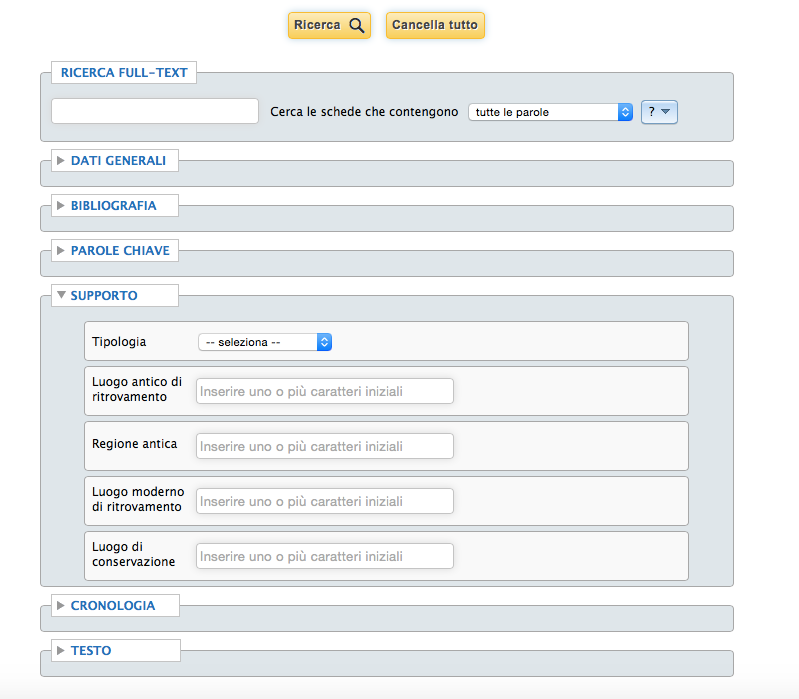
\includegraphics[width=\columnwidth]{EAGLE2016FullPaperrevised-img004.png}
\caption{Different searching categories.}
\label{fig:4}
\end{figure}








\begin{figure}[!bp]
\centering
 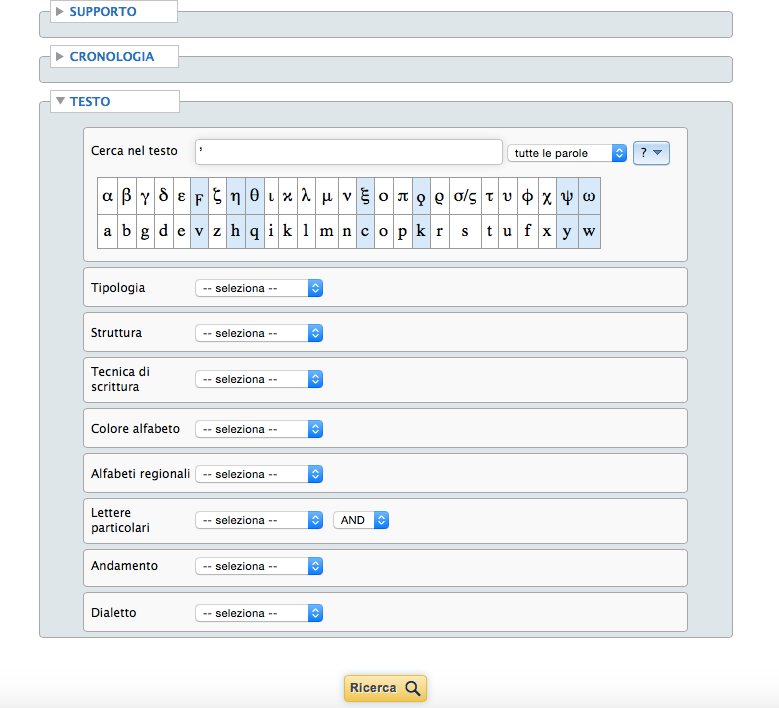
\includegraphics[width=\columnwidth]{EAGLE2016FullPaperrevised-img005.png}
\caption{Advanced text search}
\label{fig:5}
\end{figure}


Other filters will be employed for each search result. A section entitled ``tools'' will also be available, and will
include information on the entries’ structure, tables with the contents of different categories, links to Vocabularies
and websites, etc. 

\section{The AXON Project for teaching and academic research}




\subsection{Teaching}





The AXON Project, as an example of a digital edition of inscriptions (see esp. genetic lemma and apparatus) with a high
degree of clarity for contributors and users, is a useful tool for teaching Greek epigraphy as well as ancient history.
Many contributors are university lecturers / professors of Greek Epigraphy, and the scientific committee includes high
school teachers and instructors in classical languages, making AXON especially well-suited for educational purposes and
for use by students: for engaging them, for example, in the composition of entries. The interoperability of the AXON
website and the cross-references to other Digital Humanities projects are essential elements in the development of this
discipline. 







\subsection{Significance for the academic community}





Each entry is created by an expert contributor and is subject to double-blind peer review, thus assuring an important
contribution to the scholarly community. At the same time, the hyperlinks to other websites and digital editions will
make it easier for the user to check immediately all similar projects. Finally, the indexing allows for the easy
discovery and use of specific information, and will be of fundamental importance for gather together groups of
documents according to particular research needs.

In conclusion, the AXON Project aims at a collaboration of expert scholars from different fields: epigraphy, ancient
history, dialectology, archaeology, digital humanities. It can produce valuable results in the domain of the digital
editing of inscriptions and, more generally, contribute to the advancement of classical studies, opening them up to a
broader audience through the world-wide web.


\bibliographystyle{sapauth-eng}
\bibliography{../../EAGLE}

\end{document}
